% !TEX TS-program = pdflatex
% !TEX encoding = UTF-8 Unicode

% This is a simple template for a LaTeX document using the "article" class.
% See "book", "report", "letter" for other types of document.

\documentclass[11pt]{article} % use larger type; default would be 10pt

\usepackage[utf8]{inputenc} % set input encoding (not needed with XeLaTeX)

%%% Examples of Article customizations
% These packages are optional, depending whether you want the features they provide.
% See the LaTeX Companion or other references for full information.

%%% PAGE DIMENSIONS
\usepackage{geometry} % to change the page dimensions
\geometry{a4paper} % or letterpaper (US) or a5paper or....
\geometry{margin=1in} % for example, change the margins to 2 inches all round
% \geometry{landscape} % set up the page for landscape
%   read geometry.pdf for detailed page layout information

\usepackage{graphicx} % support the \includegraphics command and options

% \usepackage[parfill]{parskip} % Activate to begin paragraphs with an empty line rather than an indent
\usepackage{amssymb}
\usepackage{amsmath}
%%% PACKAGES
\usepackage{booktabs} % for much better looking tables
\usepackage{array} % for better arrays (eg matrices) in maths
\usepackage{paralist} % very flexible & customisable lists (eg. enumerate/itemize, etc.)
\usepackage{verbatim} % adds environment for commenting out blocks of text & for better verbatim
\usepackage{subfig} % make it possible to include more than one captioned figure/table in a single float
% These packages are all incorporated in the memoir class to one degree or another...

%%% HEADERS & FOOTERS
\usepackage{fancyhdr} % This should be set AFTER setting up the page geometry
\pagestyle{fancy} % options: empty , plain , fancy
\renewcommand{\headrulewidth}{0pt} % customise the layout...
\lhead{}\chead{}\rhead{}
\lfoot{}\cfoot{\thepage}\rfoot{}

%%% SECTION TITLE APPEARANCE
\usepackage{sectsty}
\allsectionsfont{\sffamily\mdseries\upshape} % (See the fntguide.pdf for font help)
% (This matches ConTeXt defaults)

%%% ToC (table of contents) APPEARANCE
\usepackage[nottoc,notlof,notlot]{tocbibind} % Put the bibliography in the ToC
\usepackage[titles,subfigure]{tocloft} % Alter the style of the Table of Contents
\usepackage{bbm}
\usepackage{endnotes}

\renewcommand{\cftsecfont}{\rmfamily\mdseries\upshape}
\renewcommand{\cftsecpagefont}{\rmfamily\mdseries\upshape} % No bold!
\DeclareMathOperator*{\argmax}{arg\,max}
\DeclareMathOperator*{\argmin}{arg\,min}
\usepackage{graphicx}
\graphicspath{ {./pings/} }

\newcount\colveccount
\newcommand*\colvec[1]{
        \global\colveccount#1
        \begin{pmatrix}
        \colvecnext
}
\def\colvecnext#1{
        #1
        \global\advance\colveccount-1
        \ifnum\colveccount>0
                \\
                \expandafter\colvecnext
        \else
                \end{pmatrix}
        \fi
}

\newcommand{\norm}[1]{\left\lVert#1\right\rVert}

\title{Econometrics HW2}
\author{Michael B. Nattinger\footnote{I worked on this assignment with my study group: Alex von Hafften, Andrew Smith, and Ryan Mather. I have also discussed problem(s) with Emily Case, Sarah Bass, Katherine Kwok, and Danny Edgel.}}

\begin{document}
\maketitle

\section{Question 1}
\subsection{Part A}
Note that, by the law of large numbers and continuous mapping theorem, $\hat{Cov}(Y,Z) \rightarrow_p Cov(Y,Z), \hat{Cov}(Z,X) \rightarrow_p Cov(Z,X)$. 
Then,
\begin{align*}
\hat{\beta}^{iv}_1 &\rightarrow_p \frac{Cov(Z,Y)}{Cov(Z,X)}\\
&=\frac{Cov(Z,\beta_0 + X\beta_1 + U)}{Cov(Z,X)}\\
&=\frac{Cov(Z,\beta_0 + X\beta_1 + U)}{Cov(Z,X)}\\
&= \frac{Cov(Z,\beta_0) + Cov(Z,X\beta_1) + Cov(Z,U)}{Cov(Z,X)}\\
&= \frac{0 + \beta_1Cov(Z,X) + Cov(Z,U)}{Cov(Z,X)}\\
&= \beta_1 +  \frac{ Cov(Z,U)}{Cov(Z,X)}
\end{align*}
Note that $Cov(U,Z) = E(UZ) - EUEZ =\\ E[ZE[U|Z]] - E[Z]E[U] = E[Z(2)] - EZE[E[U|Z]] = 2E[Z] - 2E[Z] = 0.$ Therefore, $\hat{\beta}^{iv}_1 \rightarrow_p \beta_1$.
\subsection{Part B}
By LLN and CMT,
\begin{align*}
\hat{\beta}^{iv}_0 &\rightarrow_p E[Y] - E[X]\beta_1\\
&=  E[\beta_0 + X\beta_1 + U] - E[X]\beta_1\\
&= \beta_0 + \beta_1 E[X] + E[U] - E[X]\beta_1\\
&= \beta_0 + E[E[U|Z]]\\
& = \beta_0 + 2 \neq \beta_0.
\end{align*}
Therefore, $\hat{\beta}^{iv}_0 \rightarrow_p \beta_0 + 2 \neq \beta_0.$
\section{Question 2}
\subsection{Part A}
Z is a valid instrument for X so long as Z satisfies exogeneity and relevance conditions. We are given that exogeneity is satisfied because we know that $E[U,V|Z] = 0,$ and Z is only in the second equation of the triangular form, and not the first. We are not given sufficient information to know with certainty that relevance is satisfied. This will be true if $\pi_1 \neq 0.$ This is true because of the following:
\begin{align*}
Cov(X,Z) &= Cov(\pi_0 + Z\pi_1 + V,Z)\\
&= Cov(\pi_0,Z) + Cov(Z\pi_1,Z) + Cov(V,Z)\\
&= \pi_1Var(Z) + E[VZ] + EVEZ\\
&= \pi_1Var(Z) + E[ZE[V|Z]] + EZE[E[V|Z]]\\
&= \pi_1Var(Z).
\end{align*}
\subsection{Part B}
\begin{align*}
Y &= \beta_0 + X\beta_1 + U\\
&=  \beta_0 + (\pi_0 + Z\pi_1 + V)\beta_1 + U\\
&=  \beta_0 +\pi_0\beta_1 + Z\pi_1\beta_1 + V\beta_1 + U\\
&= \gamma_0 + Z\gamma_1 +\epsilon,
\end{align*}
where $\gamma_0 = \beta_0 + \pi_0\beta_1, \gamma_1 = \pi_1\beta_1, \epsilon = V\beta_1 + U$.
\subsection{Part C}
From partitioned regression we have the following:
\begin{align*}
\hat{\gamma}_1/\hat{\pi}_1 &= \left(\sum_{i=1}^n (Z_i - \bar{Z_n})^2\right)^{-1}\left( \sum_{i=1}^n (Z_i - \bar{Z_n})(Y_i - \bar{Y}_n)\right)\left(\sum_{i=1}^n (Z_i - \bar{Z_n})^2 \right) \left(\sum_{i=1}^n (Z_i - \bar{Z_n})(X_i - \bar{X}_n) \right)^{-1}\\
&= \left(\sum_{i=1}^n (Z_i - \bar{Z_n})(Y_i - \bar{Y}_n) \right)\left(\sum_{i=1}^n (Z_i - \bar{Z_n})(X_i - \bar{X}_n) \right)^{-1}\\
&= \hat{Cov}(Z,Y)/\hat{Cov}(Z,X).
\end{align*}
This is the form of $\hat{\beta}_{iv}.$
\subsection{Part D}
We will begin from the least squares projection of $U$ onto $V$. Let $U = \delta_2 V + \xi,$ where $\delta_2 = \frac{E[VU]}{E[V^2]}$. Now, note the following:
\begin{align*}
Var(V) &= E[V^2] - E[V]^2 = E[V^2] - E[E[V|Z]]^2\\
&= E[V^2]. \\
Cov(V,U) &= E[VU] - E[V]E[U] = E[VU] - E[E[V|Z]]E[E[U|Z]] \\
&= E[VU]\\
\Rightarrow \delta_2 &= \frac{Cov(V,U)}{Var(V)}.\\
Cov(V,\xi) &= Cov(V,U-\delta_2 V)\\
&= Cov(V,U) - \delta_2 Cov(V,V)\\
&= Cov(V,U) - \frac{Cov(V,U)}{Var(V)} Var(V)\\
&= 0.\\
Cov(X,\xi) &= Cov(\pi_o + Z\pi_1 + V,\xi)\\
&= Cov(Z\pi_1,U-V\delta_2) + Cov(V,\xi)\\
&= \pi_1Cov(Z,U) - \pi_1\delta_2Cov(Z,V)\\
&= 0.
\end{align*}

Therefore, if we define $\delta_0:= \beta_0, \delta_1:=\beta_1:$
\begin{align*}
Y &= \delta_0 + X\delta_1 + V\delta_2 + \xi
\end{align*}
where $\delta_2 = \frac{Cov(V,U)}{Var(V)}, \xi = U - \delta_2V,$ and $Cov(X,\xi) = Cov(V,\xi) = 0$.
\subsection{Part E}
%Our OLS estimate is the following:
%\begin{align*}
%\hat{Y}_i &= \hat{\delta}_0 + X_i\hat{\delta}_1 + \hat{V}_i\hat{\delta}_2\\
%&=  \hat{\delta}_0 + X_i\hat{\delta}_1 + (X_i - \hat{\pi}_0 - Z_i\hat{\pi}_1)\hat{\delta}_2
%\end{align*}
As in Part C, I appeal to partitioned regression:
\begin{align*}
c_i &= 1-\hat{V}_i\left( \sum_{i=1}^n \hat{V}_i \right) \left( \sum_{i=1}^n \hat{V}_i^2\right)^{-1} = 1\\
\tilde{X}_i &= X_i - \hat{V}_i\left( \sum_{i=1}^n \hat{V}_iX_i \right) \left( \sum_{i=1}^n \hat{V}_i^2\right)^{-1}\\
&= X_i - \hat{V}_i\\
&= \hat{\pi}_0 + Z_i \hat{\pi}_1.
\end{align*}

We can now calculate our OLS estimate $\hat{\delta}_2$ as a simple regression result including the constant (as our residualized constant term remains exactly a constant term) and $\tilde{X} =\hat{\pi}_0 + Z \hat{\pi}_1 $:
\begin{align*}
\hat{\delta}_1 &= \frac{\hat{Cov}(\tilde{X},Y)}{\hat{Var}(\tilde{X})}\\
&=\frac{\hat{Cov}(\hat{\pi}_0 + Z \hat{\pi}_1,Y)}{\hat{Var}(\hat{\pi}_0 + Z \hat{\pi}_1)}\\
&= \frac{\hat{Cov}(Z \hat{\pi}_1,Y)}{\hat{Var}( Z \hat{\pi}_1)}\\
&= \frac{1}{\hat{\pi}_1}\frac{\hat{Cov}(Z ,Y)}{\hat{Var}( Z )}\\
&= \frac{\hat{\gamma}_1}{\hat{\pi}_1}\\
&= \hat{\beta}_1^{iv}
\end{align*}

The control variable estimator is equivalent to the IV estimator.

\section{Question 3}

\subsection{Part A}
$\beta_1$ is the expected change in the mother's probability of working caused by having more than 2 children in the household.
\subsection{Part B}
$X_1$ is likely to be endogenously determined. Mothers that have better jobs and work more may be more likely to prioritize their career and less likely to have more children. Additionally, mothers with more children may have less time to work. The result is a simultaneous system of endogeneous equations, and the OLS estimate is likely to overstate $X_1$'s negative effect on mother's labor supply.
\subsection{Part C}
In this case, $\beta_1$ would be the expected change in the probability that the husband worked during the year caused by having more than 2 children in the household.

As before, $X_1$ is likely to be endogenous for the same reason described in Part B, with the resulting bias in the estimated OLS coefficient being an overstatement on the negative impact on labor supply hours coming from $X_1$.

\subsection{Part D}

The two conditions $Z_1$ must satisfy to be a valid instrument for $X_1$ are relevance and exogeneity. $Z_1$ seems to me to be relevant, as it is certainly conceivable to me that parents who have two sons may want at least one daughter, and have another child to try for a daughter, or vice-versa. So, the first two children being the same sex may have some nonzero correlation with having more than two children.

In this case, one would argue that the exogeneity comes from the fact that the sex of the first two children is determined by nature. This seems hard to disagree with.
\subsection{Part E}
Below we display the regression output from Stata.

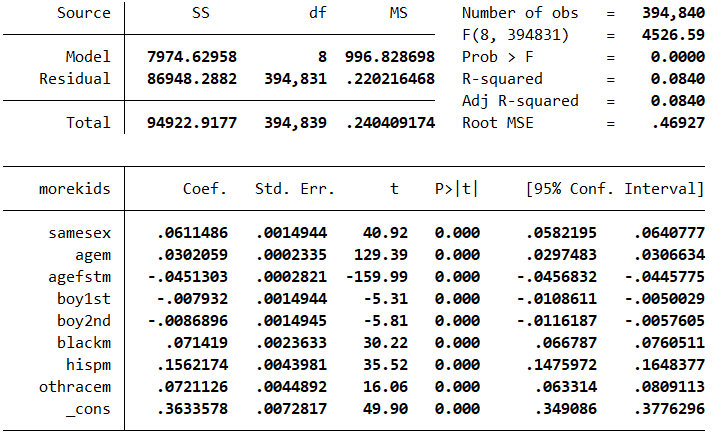
\includegraphics{hw2q4}

The regression results do indicate that samesex ($Z_1$) satisfies the relevance condition for use as an instrument for morekids ($X_1$) as the coefficient of the regression above shows that $Z_1$ has a very significantly nonzero value.

\subsection{Part F}
Below are the replication results. For all models, results are very close although in some cases the results differ very slightly.
\begin{center}
\begin{tabular}{c | c c c c c}
\hline
& All W., OLS & All W., 2SLS & M. W., 2SLS & H. of M.W., OLS & H. of M.W., 2SLS \\
\hline
Worked for pay & -.176 & -.117 & -.117 & -.007 & .004 \\
 & (.002) & (.025) & (.028) & (.001) & (.009)\\
Weeks worked & -8.978 & -5.559 & -5.272 & -.741 & .613 \\
 & (.072) & (1.118) & (1.218) & (.044) & (.598) \\
Hours per week & -6.647 & -4.547 & -4.784 & .254 & .539 \\
 & (.062) & (.954) & (1.023) & (.052) & (.702)
\end{tabular}
\end{center}

Stata do file that created the tex output is below.

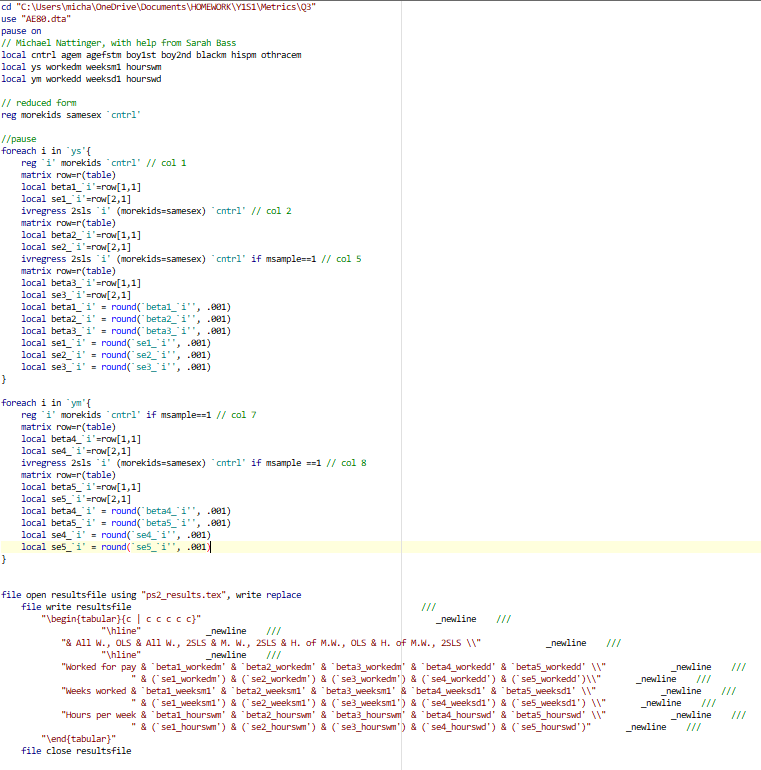
\includegraphics{hw2q5}

\end{document}
